\section{Vehicular adhoc network (VANET) attacks}
    AVs adopt two main communication mechanisms in order to communicate with the driver, other cars and the road. These are vehicle-to-vehicle (V2V) and vehicle-to-infrastructure (V2I). Figure \ref{fig:Vanet} give us an overview about VANET.
    \newline
    \begin{figure}
        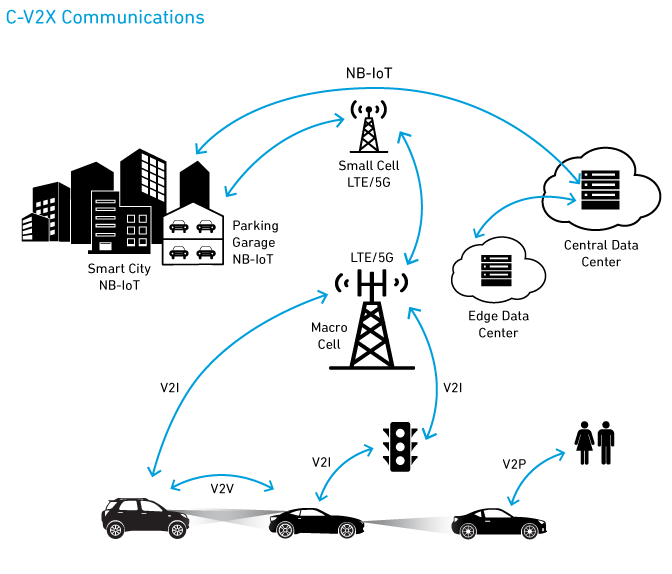
\includegraphics[width=9cm]{./files/fig2_cv2x-communications_720px.png}
        \caption{VANET network.}
        \label{fig:Vanet}
    \end{figure}
    \newline
    V2V communication provide the possibility for vehicles to communicate with each other in a peer-to-peer mechanism. This system uses the IEEE 802.11p protocol where the principle is that when two or more vehicles are in radio communication range, they can connect automatically and establish an ad hoc network where all connected nodes can share information such as position, speed, direction, etc.
    \newline
    V2I communication provide the possibility to connect vehicles to electronic devices in order to control and monitor the physical environment where they are travelling. The informations exchanged between vehicle and infrastructure can be used to optimise the traffic control, to maximise the traffic flow, minimise the fuel usage and control the pollution.

    \subsection{Authenticity/identification attacks}
    Any flaws in the process of authentication/identification may cause serious consequences to the entire network. Cryptographic scheme allows the receivers to verify the origin of the exchanged data. Some examples of authenticity attacks and their corresponding countermeasures are as follows:
    \begin{itemize}
        \item \textit{Sybil attack} is an attack where a malicious vehicle transmits the various messages with multiple fake or stolen source identities to other nodes in the network with a spoofing attack. Therefore legitimate/authenticated nodes consider the malicious messages to be legitimate and cannot detect the real identities of the attackers [26].
        \newline
        Chen et al. [27] proposed a ‘Robust Sybil Attack Detection’ approach based on motion trajectories differences of vehicles. The author has assumed that people driving vehicles on their individual path, chosen speed, and maintains some distance from other vehicular nodes for traffic or passenger safety. Therefore, each vehicle can detect attacks independently with little support from infrastructure. In this approach, infrastructures are made available vehicle’s digital signatures along with timestamp periodically or on-demand. Each motor vehicle is able to independently record these signatures and utilize them during the measure and compare the differences from neighboring node’s signature vectors to detect Sybil nodes.
        \newline
        Another countermeasure for this type of attack is the one proposed by Park et al. in [28]. Basically, in this approach when a vehicle passes through an intelligent traffic infrastructure it acquires certified timestamp that is signed by the infrastructure. A motor vehicle sent a traffic message, which contains a timestamp series to confirm thatwhen a vehicle passes through the last few infrastructures. It is unusual to have two vehicles passing through multiple infrastructures at the similar time, because each vehicles moves with different dynamics. Based on this fact, when a receiver vehicle receives numerous messages with same timestamp series can be detected as Sybil Attack.
        \newline
        This type of attack is well known by the research community and a lot of countermeasures has been developed, [29], [30], [31], we can consider it largely mitigated. 
        
        \item \textit{Replication attack} means one or more nodes claiming an legitimate identity with duplicate keys/certificates.
        J.L. Huang et al. in [32] presented an anonymous batch authenticated and key agreement (ABAKA) scheme to authenticate multiple requests sent from different vehicles and establish different session keys for different vehicles at the same time. ABAKA can efficiently authenticate multiple requests by one verification operation and negotiate a session key with each vehicle by one broadcast message. Elliptic curve cryptography is adopted to reduce the verification delay and transmission overhead. The security of ABAKA is based on the elliptic curve discrete logarithm problem, which is an unsolved NP-complete problem.
        \newline
        Y. Hao et al. in [33] proposed a new cooperative message authentication protocol (CMAP) with an assumption that each safety message carries the location information of the sender vehicle (which can be generated by a global positioning system (GPS) device). Verifiers of each message are defined according to their locations in relation to the sender. Only the selected verifiers check the validity of the message while other vehicles rely on verification results from these verifiers. In the test phase of the protocol it result to be the most effetive one for counter the replication attack.
        \newline 
        Also in this case  we can consider this attack fully mitigated. 
    \end{itemize}
    
    \subsection{Availability attacks}
    The requirement of availability is mandatory to ensure the safety of the involved drivers and vehicles. Due to the major impact on the network resources, DoS attacks are commonly recognized as the most serious threat to the availability of vehicle related systems. Authentication, detection and cryptographic solutions are usually employed to counter such attacks.
    \begin{itemize}
        \item \textit{Malware attack} is to jeopardize the network or software components of the system via any form of hostile or intrusive software like computer viruses. Such attack can be mitigated by using anti-malware software and firewall.
        
        \item \textit{Denial of Service (DOS) attack} has the major purpose to prevent legitimate entities from accessing the network services and resources. Basically, denial-of-service attack means that an adversary floods the  target  with  requests, overloading its resources to disrupt availability.It can also be known as DDOS (Distributed Denial of Service), when multiple computers and/or Internet connections are used to launch the attack. Researchers have demonstrated how DDoS attacks can be performed against VANETs [34] and that it is possible to identify malicious connections for prevention [35], [36], [37]. Different types of DoS attacks can be performed by overwhelming a single network node, V2V or V2I.
        \newline
        He et al. propose a pre-authentication scheme, which taking advantage of the one way hash chain and a group re-keying method to mitigate DoS attack in [38]. 
        \newline
        Verma et al. designs a data structure to filter packets and detect abrupt change, thereby avoiding DoS attack in [39].
        \newline
        This type of attack is well known by the research community and a lot of countermeasures has been developed so we can consider it fully mitigated. 
        
        \item \textit{Wormhole attack} means that the packets captured at one region of the network are transmitted to another region of the network. This would confuse the routing mechanisms where the accuracy of the distance between entities inside the network is crucial [39]. 
        \newline 
        S.M. Safi et al. in [40] propose a way to restrict the packet’s maximum allowed transmission distance, which would ensure that the recipient of the packet is within reasonable range of the sender. This method, called HEAP, is very suitable for VANETs because it has a better performance compared to other authentication methods. HEAP is applicable for all unicast, multicast, and broadcast applications. We can also use HEAP as authenticator for all types of packets.
    \end{itemize}
    
    \subsection{Data integrity attacks}
    Data integrity refers to the fact that the data must be intact and unchanged throughout its lifecycle. The attackers especially those having authenticated entities could easily alter the data or create false data. Thus, secure communication and information encryption are necessary to prevent/mitigate the attacks on data integrity.
    \begin{itemize}
        \item \textit{Masquerading attack} means any attack that uses a forged identity to gain unofficial access to the system. For example, a malicious node disguises itself as an emergency vehicle, and so the surrounding vehicles are tricked into slowing down, changing lane, etc. in order to give way to it.
        \newline 
        T.W. Chima et al. in [41]  proposes a scheme, called SPECS (Secure and Privacy Enhancing Communications Schemes), to ensure the security and privacy issues of V2V communications and detect the masquerading attacks. This approach is based on the idea of IBV (Identity-Based Batch Verification) Scheme [42], which suffers from impersonation attack and cannot fulfill privacy requirements. To protect the identity of each vehicle it uses pseudo-identity and a shared secret key \textit{m} between a vehicle and RSU (Road-Side Unit).
        \newline
        To authenticate a vehicle with a nearby RSU, the scheme uses Public Key Infrastructure (PKI) and assumes that there is a trusted authority (TA) constantly online. A secure fixed network is dedicated for communications between RSUs and TA. To avoid bottleneck, redundant TAs with identical functionalities and databases are installed. It is worth noting that TA is the only authorized component knowing the real identity of vehicles. The vehicle authentication with the TA is performed via RSU. Then TA passes verification information to RSU. RSU then generates a shared secret key mi with the vehicle. If this is the first time that the vehicle authenticates itself with the TA, TA will also pass its master key \textit{s} and a shared secret \textit{m} to the vehicle, via RSU of course. This only needs to be done once in the whole journey. For security reasons, \textit{s} is not preloaded into any vehicle’s hardware. Each time the vehicle passes a new RSU, a new shared-secret key is generated. To generate the signature, vehicle uses the shared secret key and hash function with the signing key. As \textit{m} is only known by the vehicle, RSU and TA, attackers or other vehicles cannot generate the valid signing key to sign the message. RSU always verify the vehicle’s signature even if the vehicle uses pseudo identity to sign the message. Invalid signatures can be detected using a batch verification process by RSU. In IBV (Identity-Based Batch Verification), if any invalid signature is found using the batch verification process the whole batch is dropped.
        \newline
        If an attacker is found, it notifies other vehicles and repeats the process until the search reaches a predefined level or all signatures are validated. After verifying the signature, the RSU broadcasts the message to all vehicles without the hash value, which is stored into positive and negative bloom filters. Any vehicle that wants to know the validity of a received message will create the hash value and compare with the bloom filters hash value. A message is valid if the hash value of this message is found in the positive bloom filter. Otherwise, the message is considered as invalid.
        
        \item \textit{Replay attack}, also known as \textit{Playback attack}, is an attack where data are fraudulently repeated or delayed. State-of-the-art security architectures employing a strong cryptographic system have the potential to effectively thwart application layer attacks in the case where the adversary is an untrusted outsider. Digital signatures provide data integrity for beacon messages and protect them from unauthorized change. Moreover, using nonce in the messages, which is an arbitrary number (chosen in a pseudo-random process) used only once in communication, is a technique to prevent replay attacks [43].
        \newline
        But if we consider the scenario where the adversary is a trusted insider such as a compromised vehicle with a valid certificate, the problem is much harder to solve. Typical approaches to handling this issue are via misbehavior/anomaly detection techniques such as [44], which require multiple sources of data that may not always be available. In addition, such techniques do not guarantee perfect detection in all circumstances, and are usually associated with finite false negative and false positive rates. There is much left to be done in the anomaly detection field to ensure acceptable performance of these algorithms to ensure the safety of passengers.
    \end{itemize}
    
    \subsection{Confidentiality attacks}
    The attacks on confidentiality may not affect safety as previous mentioned attacks do. Nevertheless, the sensitive information exchanged in network, e.g., AVs location, ITS safety messages and driver's personal information, should be protected. Information encryption and secure communication can be used to avoid information leak.
    \begin{itemize}
        \item \textit{Eavesdropping attack:} vehicles periodically broadcast beacons that contain various types of information such as vehicle identity, current vehicle position, speed and acceleration. The availability of this information can comprise the privacy. The adversary can carry out an eavesdropping attack, to extract valuable information about the vehicle stream such as its trace by linking position data, and use it for her own benefit. 
        \newline
        Eavesdropping is a type of passive attack, and hence is difficult to detect, especially in broadcast wireless communication. However, it is possible to prevent the success of eavesdropping by using encryption to achieve data privacy or using anonymity techniques to achieve identity and location privacy. Anonymity is typically implemented using group signatures [45] or short-term certificates (pseudonyms) [46].
    \end{itemize}
    
    \subsection{Vehicle-to-pedestrian (V2P) network}
    The use of smartphones in a road context by drivers and Vulnerable Road Users is rapidly increasing. To reduce the risks related to the influence of smartphone usage in a situation where traffic needs to be considered, a collision prediction algorithm is proposed based on Pedestrian to Vehicle (P2V) and Vehicle to Pedestrian (V2P) communication technologies. A. Hussein et al. in [47] develped this algorithm that using GPS and magnetometer form a pedestrian smartphone and GPS and other sensor on AV can predict the collision angle. 
    \newline
    Figure \ref{fig:Collision} give us an overview of how the algorithm work.
    \begin{figure}
        \centering
        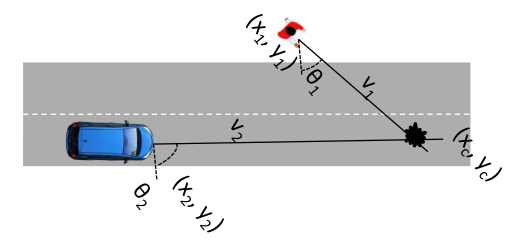
\includegraphics[width=9cm]{./files/Schermata da 2020-02-18 10-20-30.png}
        \caption{Collision prediction angle.}
        \label{fig:Collision}
    \end{figure}
    \newline
    When a collision is calculated a warning message is sent to the pedestrian and to the AV in order to replan the mission and avoid the accident. 
    \newline
    V2P communication is a new research field and not enough work has been done to make this communication safty and resilient. The future is a world where all devices are connected and now a days there are many security issue that makes the "internet of things" not safe enough. 